% !TEX root = ../entropy.tex

\section{Methods}%
\label{sec:methods}


\subsection{Dataset description}
\label{par:dataset_description}

We use data from Money Dashboard (MDB), a financial management app that allows
its users to link accounts from different banks to obtain an integrated view of
their
finances.\footnote{\href{https://www.moneydashboard.com}{https://www.moneydashboard.com}.}
The dataset contains more than 500 million transactions made between 2012 and
June 2020 by about 250,000 users, and provides information such as date,
amount, and description about the transaction as well as account and user-level
information.

The main advantages of the data for the study of consumer financial behaviour
are its high frequency, that it is automatically collected and updated and thus
less prone to errors and unaffected by biases that bedevil survey measures, and
that it offers a view of consumers' entire financial life across all their
accounts, rather than just a view of their accounts held at a single bank,
provided they added all their accounts to MDB. The main limitation is the
non-representativeness of the sample relative to the population as a whole.
Financial management apps are known to be used disproportionally by men,
younger people, and people of higher socioeconomic status
\citep{carlin2019generational}. Also, as pointed out in
\citet{gelman2014harnessing}, a willingness to share financial information with
a third party might not only select on demographic characteristics, but also
for an increased need for financial management or a higher degree of financial
sophistication. Because our analysis does not rely on representativeness, we do
not address this.\footnote{For an example of how re-weighing can be used to
mitigate the non-representative issue, see \citet{bourquin2020effects}.}


\paragraph{Data issues}%
\label{par:data_issues}

\citet{bourquin2020effects} argue that because some of the accounts in the data
will be joint accounts, units of observations should be tought of as
"households" rather than "users". We do not agree that this is the most prudent
approach. The validity of thinking of units as households depends on the
proportion of users in the data who add joint accounts and on the proportion of
transactions -- out of a user's total number of transactions -- additionally
observed as a result. Given that the sample is skewed towards younger
individuals we think it is unlikely that a majority of them has added joint
accounts. Furthermore, it seems reasonable to assume that in most cases, joint
accounts are mainly used for common household expenditures similar that are
similar to those of a single user (albeit in higher amounts), and are thus
unlikely to alter the observed spending profile much. Thus, we think of units
of observations as individuals, not households. 

Some accounts might be business accounts. Using versions of the algorightms
used by \citet{bourquin2020effects} to identify such accounts showed, however,
that such accounts only make up a tiny percentage of overall accounts and would
not influence our results. We thus do not exclude them.


\subsection{Preprocessing and sample selection}%
\label{par:preprocessing_and_sample_selection}

We restrict our sample to users for whom we can observe a regular income, can
be reasonably sure that they have added all their bank account to MDB, and for
whom we observe at least six months of data. Table~\ref{tab:selection}
summarises the sample selection steps we applied to a 1 percent sample of the
raw data, associated data losses, and the size of our final sample.

\begin{table}[H]
\centering
\caption{Sample selection}\label{tab:selection}
\begin{tabular}{lrrrr}
\toprule
                                       &  Users & User-months &       Txns & Txns (m\pounds) \\
\midrule
                            Raw sample & 27,175 &     795,338 & 65,972,558 &          12,527 \\
             Drop first and last month & 26,565 &     741,170 & 64,157,932 &          12,179 \\
             At least 6 months of data & 23,238 &     732,499 & 63,592,713 &          12,074 \\
          At least one savings account & 14,315 &     473,814 & 43,983,467 &           8,898 \\
          At least one current account & 14,028 &     466,827 & 43,408,017 &           8,792 \\
At least \pounds5,000 of annual income &  5,335 &     159,663 & 16,815,335 &           3,339 \\
           At least 10 txns each month &  4,789 &     142,602 & 15,328,431 &           3,023 \\
  At least \pounds200 of monthly spend &  4,175 &     122,174 & 13,592,387 &           2,713 \\
      Complete demographic information &  3,417 &     104,660 & 11,689,245 &           2,299 \\
                       Drop test users &  3,410 &     104,307 & 11,638,106 &           2,292 \\
                           Working age &  3,345 &     102,302 & 11,465,704 &           2,241 \\
                          Final sample &  3,345 &     102,302 & 11,465,704 &           2,241 \\
\bottomrule
\end{tabular}

\end{table}


\subsection{Dependent variables}
\label{sub:dependent_variables}

Identifying savings transactions: We classify as payments into savings accounts
all savings account credits of \pounds5 or more that are not identified as
interest payments or automated "save the change" transfers (similarly for
debits).\footnote{While standing order transactions are unlikely to be related
to entropy in the short-run, we do not exclude such transactions since, best we
can tell, the only account for a small fraction of total transactions.} 

Dummy for savings txn in current month. Motivation: \citet{mps2018building} finds that
saving habit is often more important than amount saved.


\subsection{Spending profiles}%
\label{sub:spending_profiles}

We define a user's spending profile as the distribution of the number of
spending transactionas across different spend categories. To summarise these
distributions, we calculate spending entropy, based on the formula proposed by
\citet{shannon1948mathematical}, who defines entropy as $H =
-\sum{p_i}log(p_i)$, which sums, for all possible events, the product of the
probability of an event $i$ occuring with the logarithm of that
probability.\footnote{Shannon entropy is customarily denoted as $H$ following
    Shannon's own naming after Ludwig Boltzman's 1872 H-theorem in statistical
    mechanics, to which it is analagous.} The base the logarithm is often
    chosen to be 2, though other choices are possible.\footnote{The choice of
        the base for the logarithm varies by application and determines the
        units. Base 2 means that information is expressed in bits. The
natural logarithm, another popular choice, expresses information in
\textit{nats}.} Entropy is a cornerstone of information theory, where it
measures the amount of information contained in an event. In the behavioural
sciences, behavioural entropy has recently been shown to predict the frequency
of grocery visits and the per-capita spend per visit
\citep{guidotti2015behavioral}, the amount of calories consumed
\citep{skatova2019those}, and the propensity for financial distress
\citep{muggleton2020evidence}. In our context, we define the entropy of a
user's spending profile in a particular period as:\footnote{We omit individual
and time subscripts to keep notation simpler.}

\begin{equation}
\label{equ:entropy}
H = -\sum_{c \in \setc}{p_c}log(p_c),
\end{equation}

\noindent where $\setc$ is the set of all spending categories, $p_c$ the
probability that an individual makes a purchase in spending category $c$, and
$log$ the base 2 logarithm. Higher entropy means that transactions are more
equal across different spending categories, which makes it hard to predict the
next transaction, whereas low entropy profiles have the bulk of transactions in
a few dominant categories (such as groceries and transportation) and have
relatively few transactions in other categories.\footnote{For further
discussion on how to interpret Equation~\ref{equ:entropy}, see
Appendix~\ref{sec:interpreting_entropy}.} For simpler interpretation of our
regression coefficients below, we standardise entropy scores to have a mean of
0 and a standard deviation of 1.

We calculate entropy based on three sets of spend categories. The first measure
is based on 9 spending categories used by
\citet{muggleton2020evidence}.\footnote{The precise mapping from MDB
    transaction tags into these 9 categories is available on
\href{https://github.com/fabiangunzinger/entropy/blob/7fa9c565bf8959ea92a9d4fe2245da0864e19c27/src/data/txn_classifications.py\#L249}{Github}.}
The second measure is based on our own, more fine-grained, categorisation into
48 different categories.\footnote{The precise mapping from MDB transaction tags
into these 48 categories is available on
\href{https://github.com/fabiangunzinger/entropy/blob/7fa9c565bf8959ea92a9d4fe2245da0864e19c27/src/data/txn_classifications.py\#L503}{Github}.}
The third measure is based on merchant names, as labelled by Money Dashboard.

We also calculate spending category probabilities in two different ways. To
calculate what we call ``unsmoothed'' entropy scores, we calculate the $p_c$s
in Equation~\ref{equ:entropy} as simple frequentist probabilities

\begin{equation}
    p_c = \frac{f_c}{F},
\end{equation}

\noindent where $f_c$ is the number of transactions in spend category $c$ (the
frequency with which $c$ occurs) and $F = \sum_{c \in \setc}f_c$ the total
number of spending transactions. To avoid taking the log of zero for categories
with zero transactions, the sum in Equation~\ref{equ:entropy} is taken over
categories with positive transaction counts only.\footnote{This is
    automatically handled by the entropy
    \href{https://docs.scipy.org/doc/scipy/reference/generated/scipy.stats.entropy.html}{implementation}
of Python's SciPy package, which is what we use to calculate entropy scores.}
To calculate ``smoothed'' entropy scores, we apply additive smoothing to
calculate propabilities as

\begin{equation}
    p_c^{s} = \frac{f_c + 1}{F + |\setc|},
\end{equation}

\noindent where the size of set $\setc$, $|\setc|$, is the number of unique
spending categories. Hence, additive smoothing simply adds one to the numerator
and the number of unqiue spending categories to the denominator of the
unsmoothed probabilities. Because categories with a zero transaction count will
have a numerator of 1, the sum in Equation~\ref{equ:entropy} will be taken over
all categories.

One way to think of entropy is as a function of a number of simple components,
and we can rewrite Equation~\ref{equ:entropy} in a way that makes this
transparent. Let $\setcp = \{c: f_c > 0\}$ be the set of all spending
categories with positive frequency counts (i.e.  with at least one transaction)
and $\setcz = \{c: f_c = 0\}$ the set of all spending categories with a zero
frequency count. Then, using our definitions of unsmoothed and smoothed
probabilities above, we can write unsmoothed entropy as

\begin{equation}
\label{equ:entropy_us}
H = -\sum_{c \in \setcp}{\left(\frac{f_c}{F}\right)
log\left(\frac{f_c}{F}\right)},
\end{equation}

and smoothed entropy as:

\begin{equation}
\label{equ:entropy_us}
H^s = -\sum_{c \in \setcp}{\left(\frac{f_c + 1}{F + |\setc|}\right)
log\left(\frac{f_c + 1}{F + |\setc|}\right)}
+ |\setcz|\left(\frac{1}{F + |\setc|}\right)
log\left(\frac{1}{F + |\setc|}\right),
\end{equation}

\noindent where the size of set $\setcz$, $|\setcz|$, is the number of all
spending categories in which a user makes no transactions in a certain period.
These expressions make clear that, by definition, unsmoothed entropy is a
function of frequency counts of categories with positive counts only to avoid
taking logs of 0, while smoothed entropy has two parts: the additively smoothed
unsmoothed entropy, plus a constant term for each spending category with a zero
frequency count.

The expressions also make transparent the three main components of both types
of entropy: the number of spending categories with a non-zero frequency count
(and its complement, the number of categories with a zero frequency count), the
variation in the frequency counts of those categories, and the total number of
transactions ($F$).\footnote{The number of total spending categories,
    $|\setc|$, also implicitly determines unsmoothed entropy (since it
    ``scales'' the number of categories with a positive frequency count,
$|\setcp|$) and explicitly determines smoothed entropy, but it is fixed across
users and periods and does not depend on user behaviour.}

\begin{figure}[h]
    \centering 
    \caption{Correlation of entropy with its components}
    \label{fig:entropy_components}
    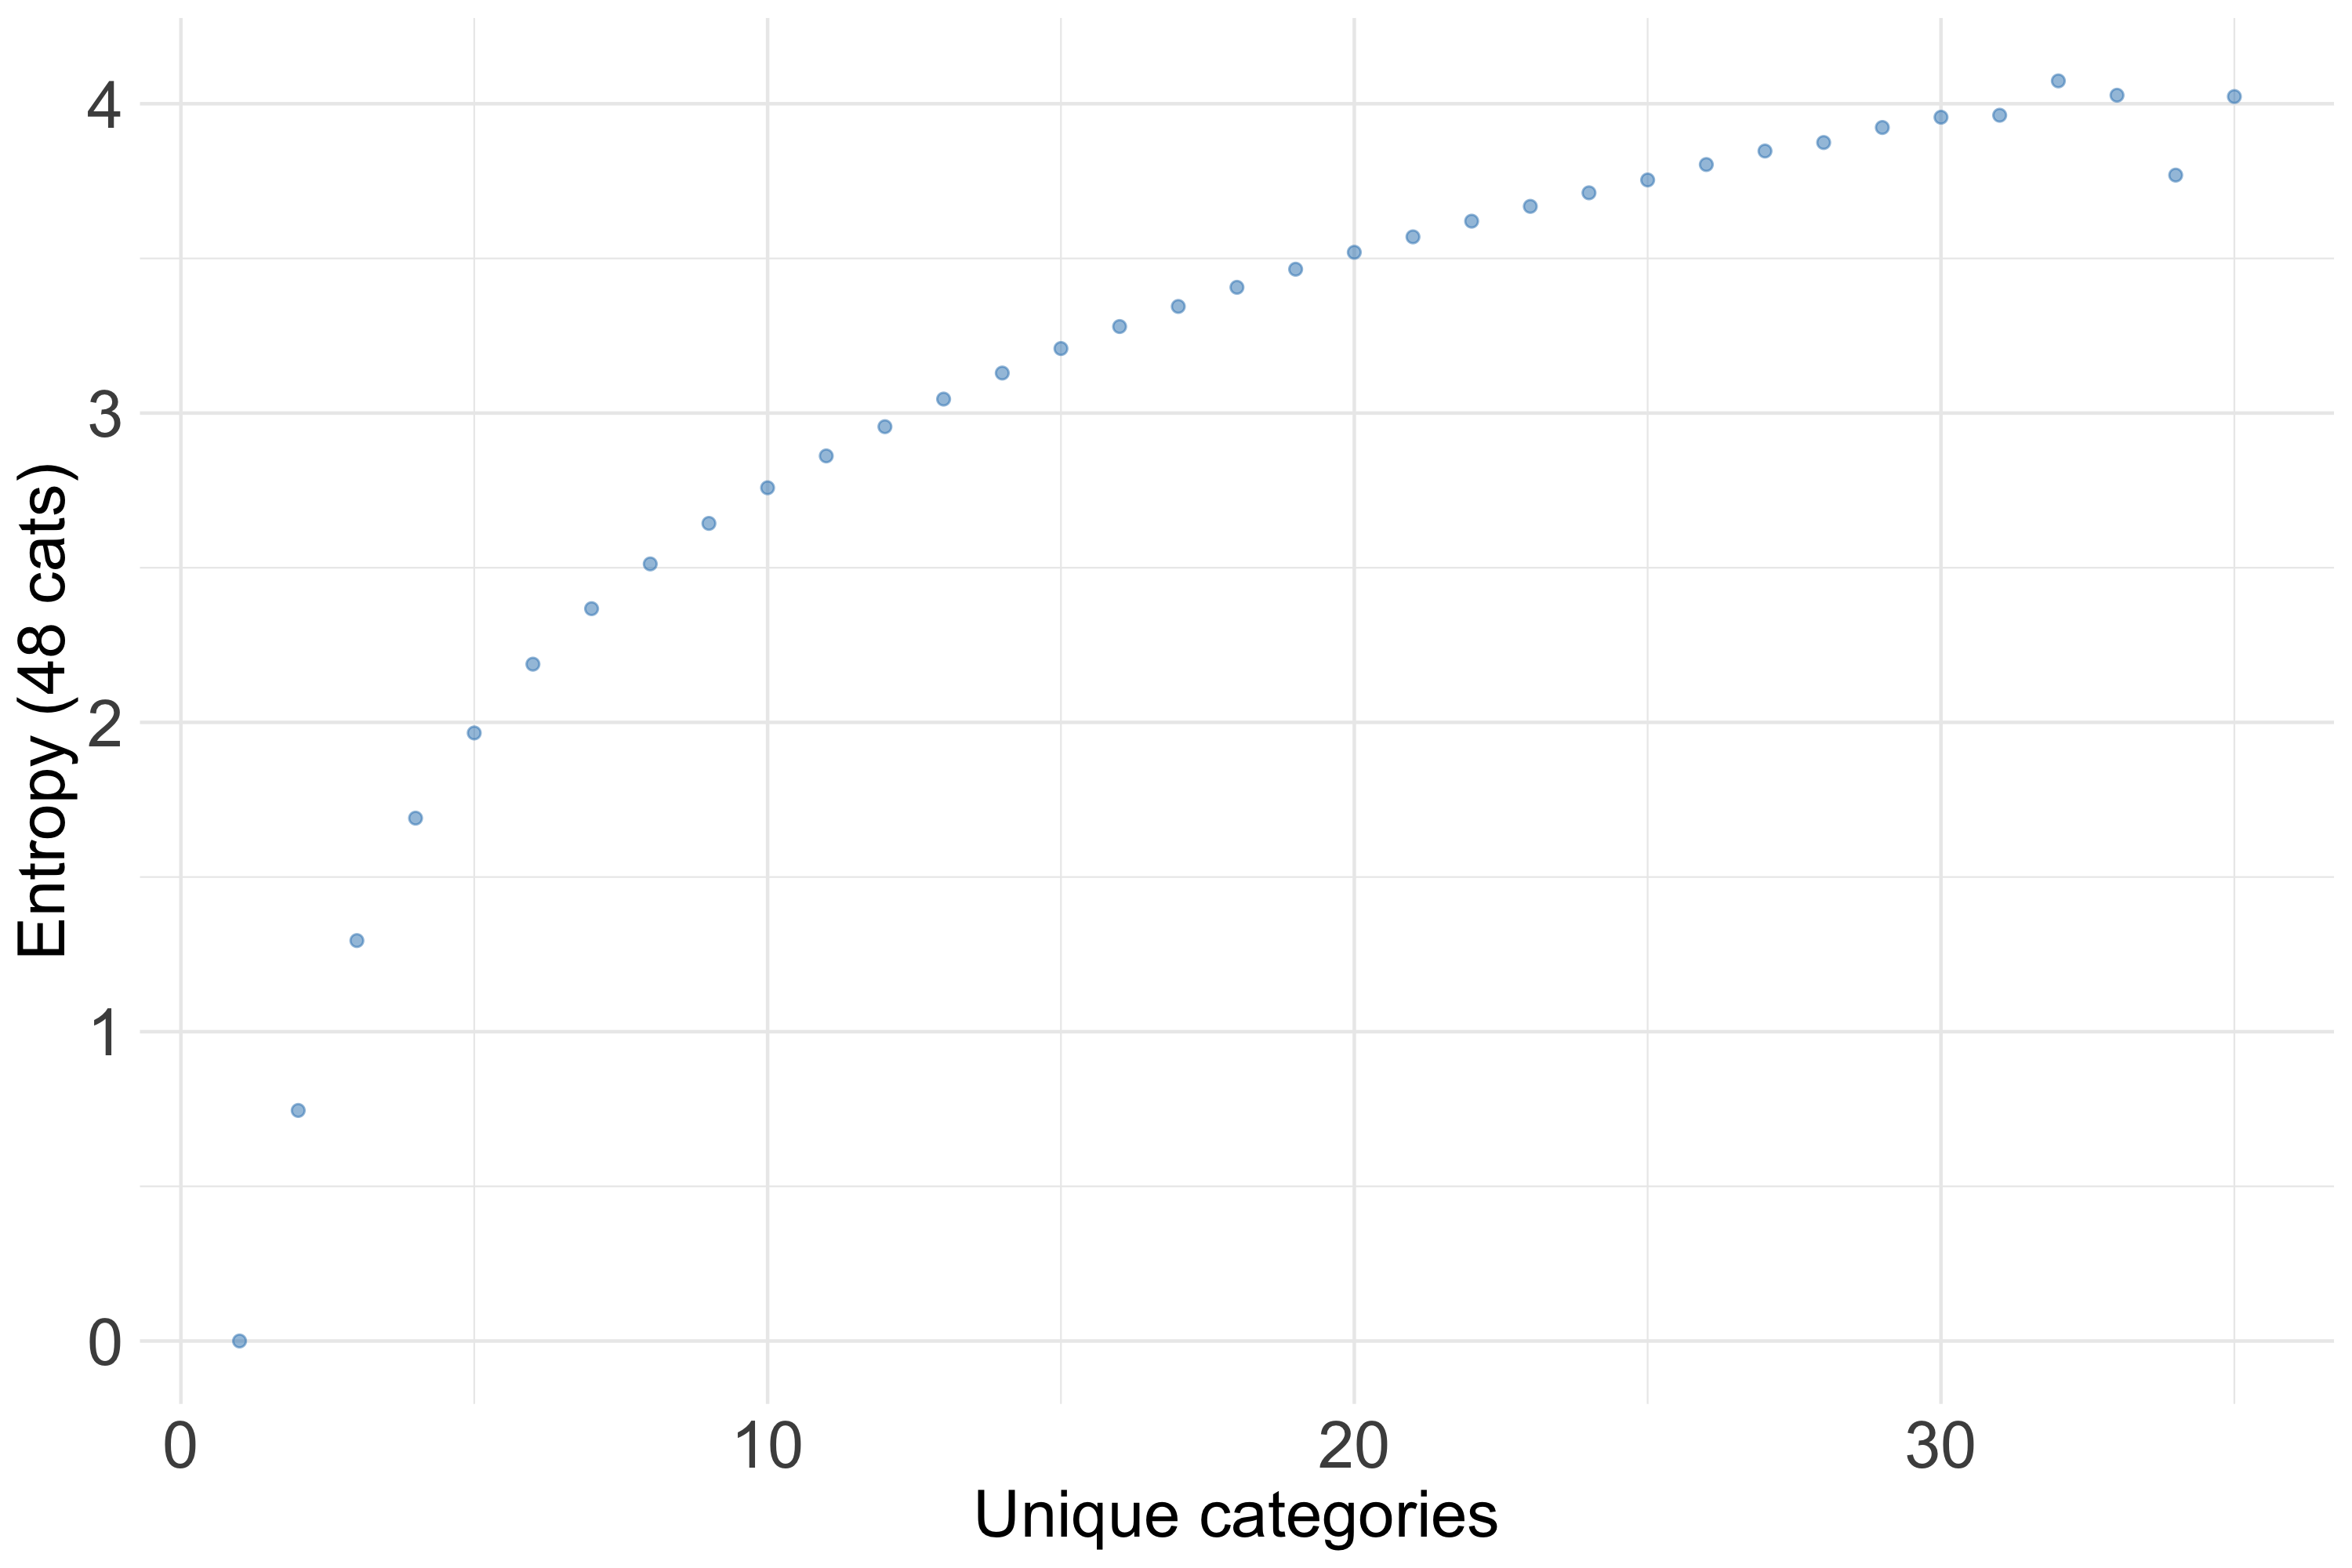
\includegraphics[width=.32\textwidth]{\figdir/scatter_entropy_nunique_tag_spend.png}
    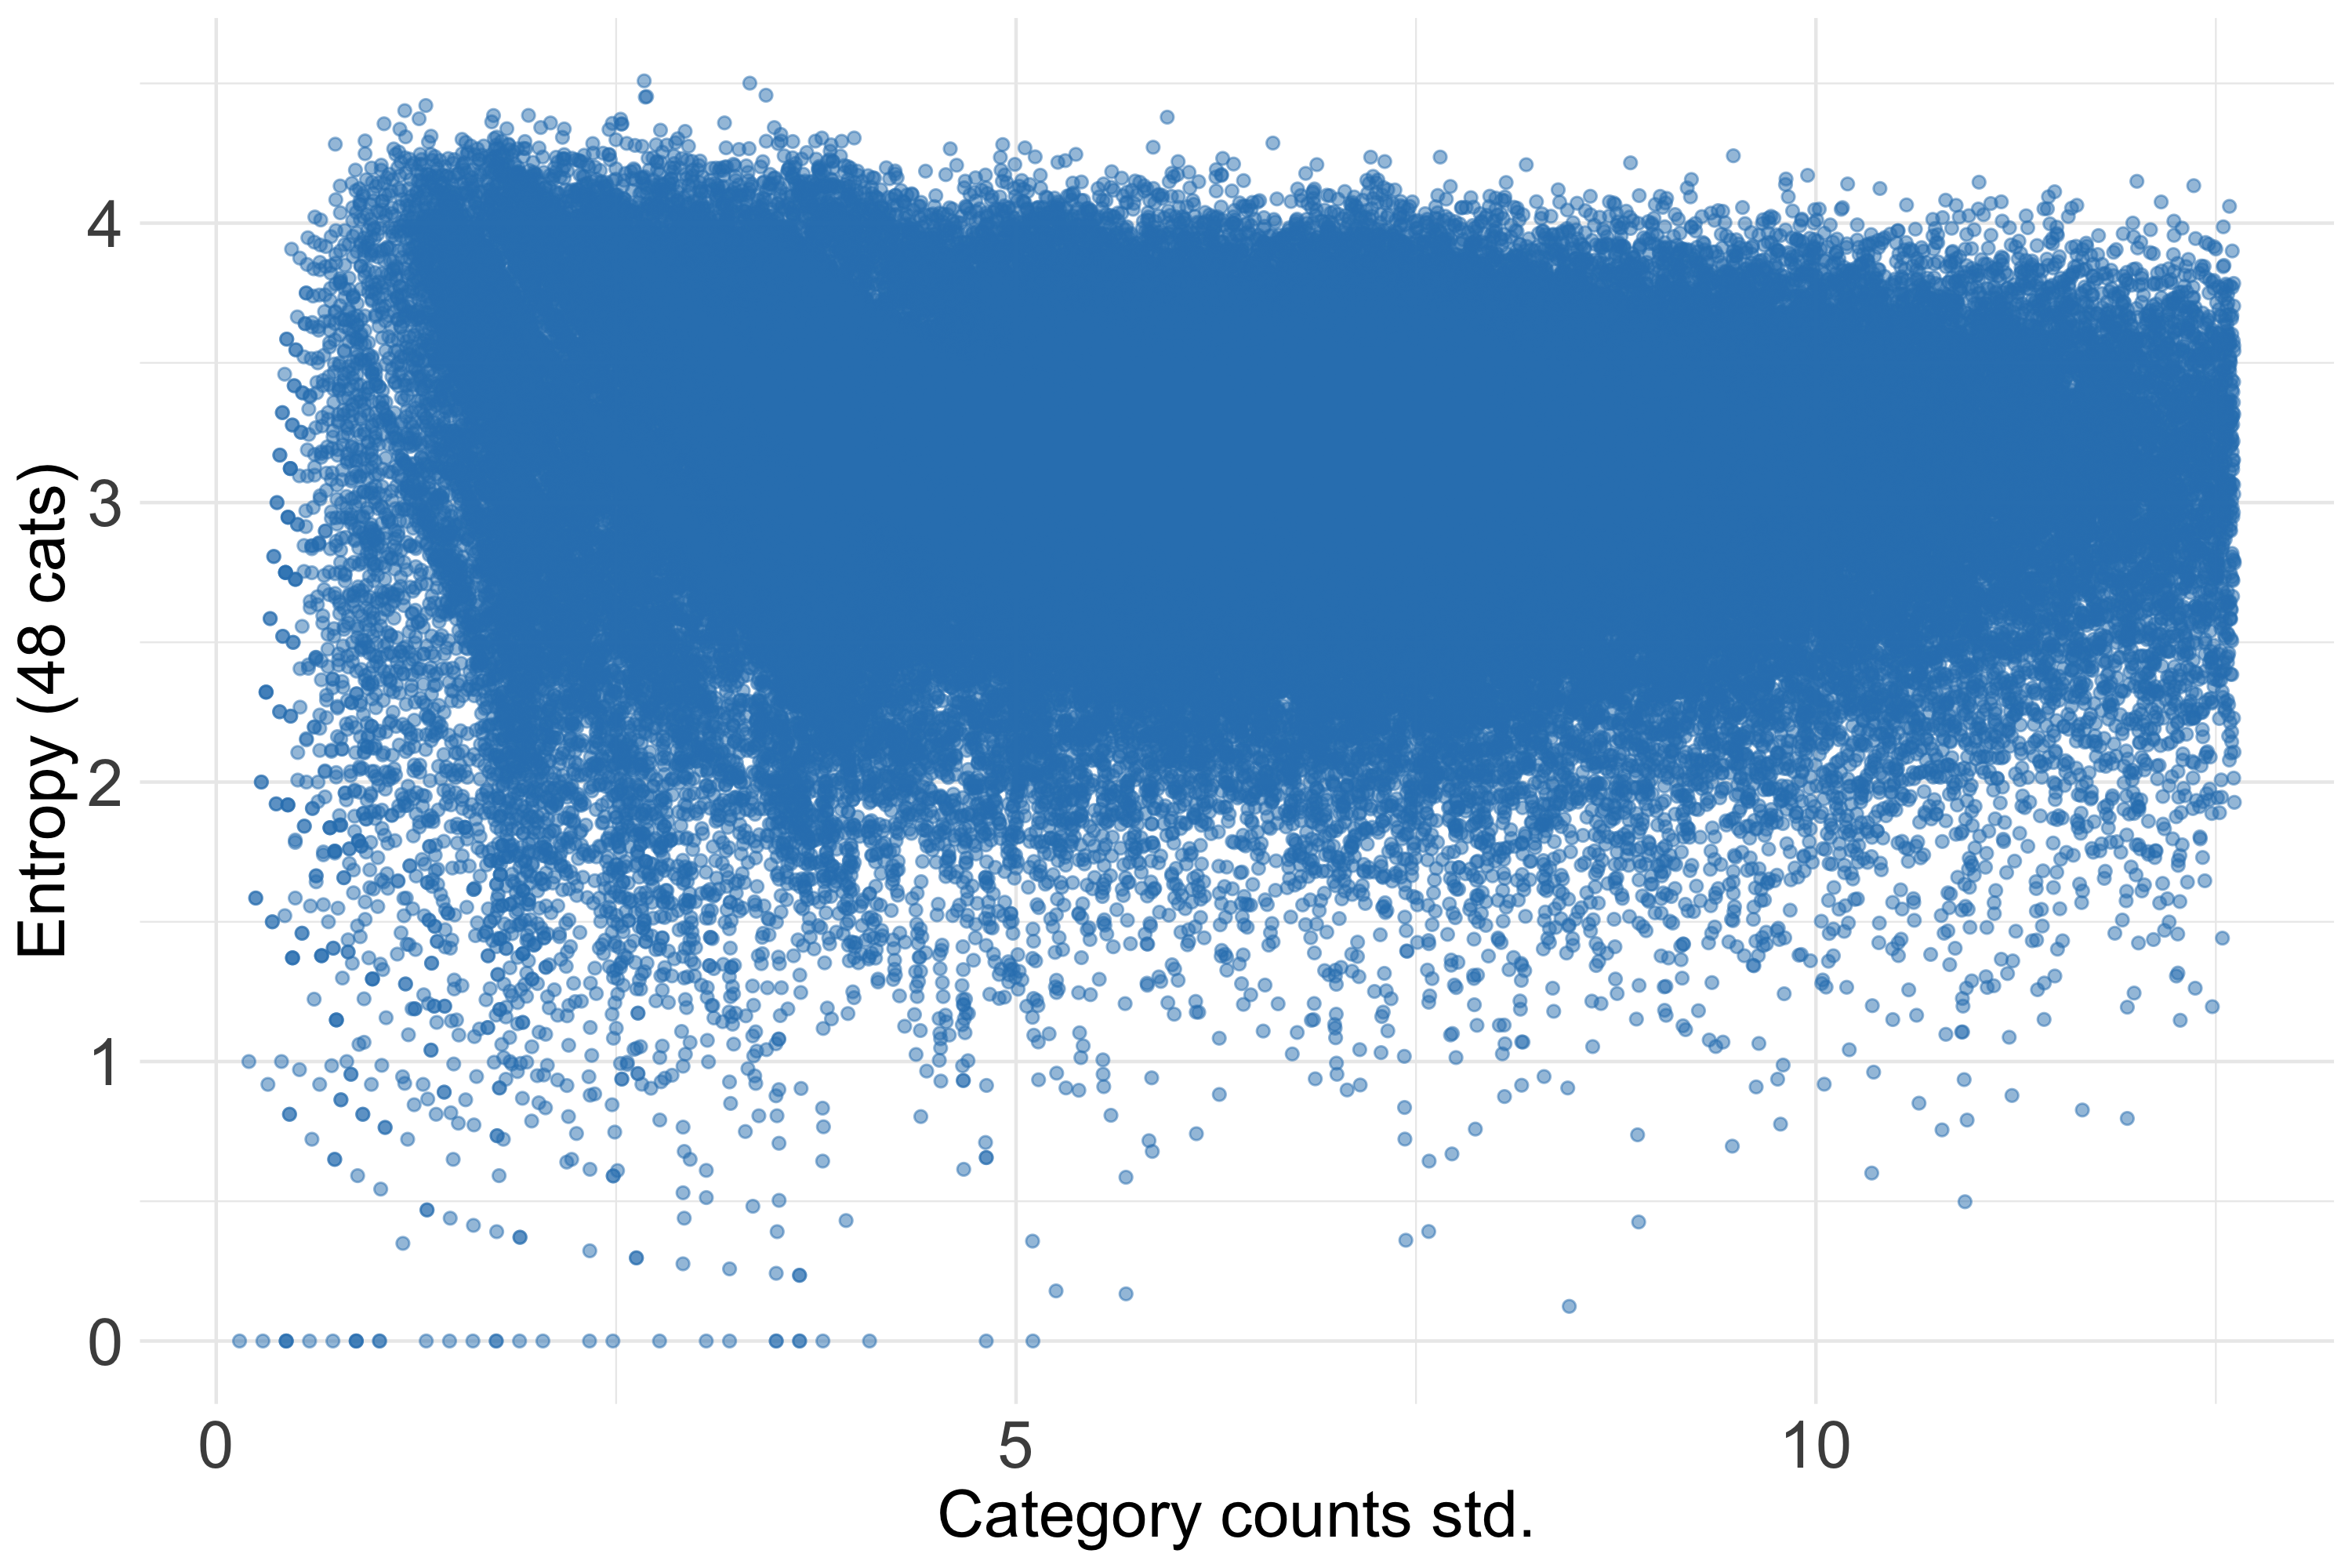
\includegraphics[width=.32\textwidth]{\figdir/scatter_entropy_std_tag_spend.png}
    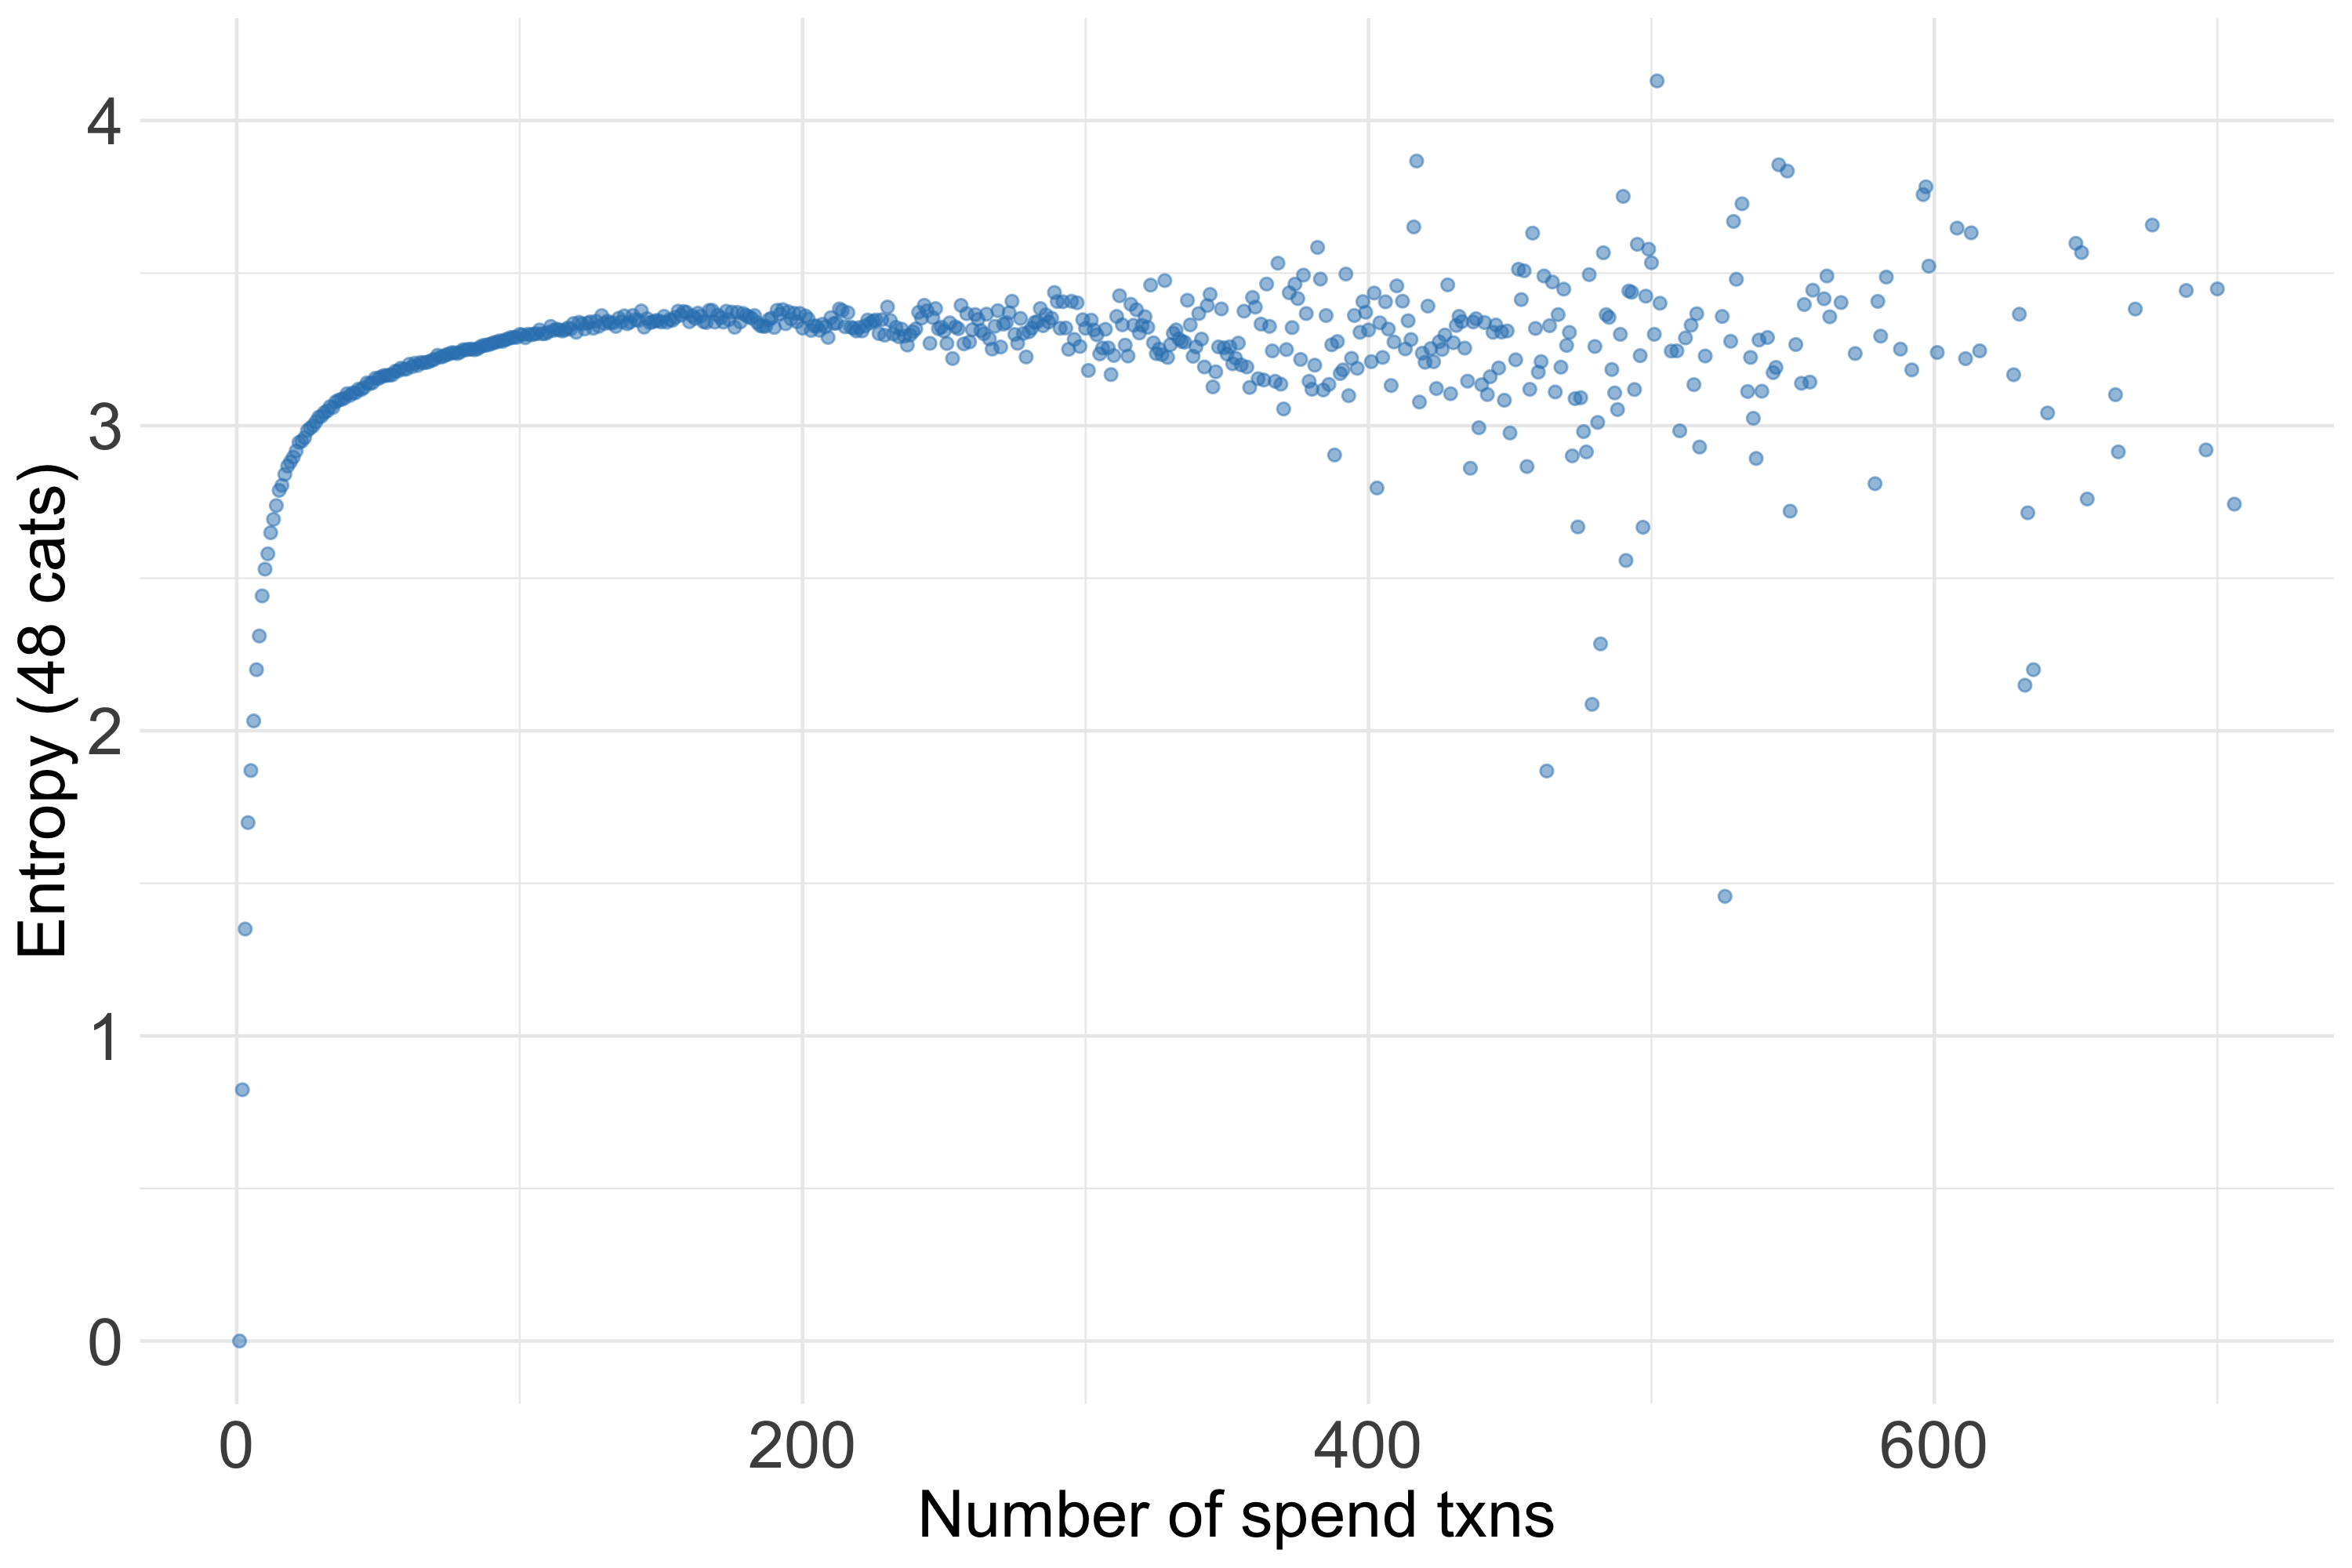
\includegraphics[width=.32\textwidth]{\figdir/scatter_entropy_txns_count_spend.png}
    \fignote{\textwidth}{Correlation of 48-categories-based unsmoothed entropy
    with its three main components: the number of unique spending categories
with positive frequency counts (left), the standard deviation of those
frequency counts (middle), and the number of total spend transactions (left).}
\end{figure}

Figure~\ref{fig:entropy_components} shows the empirical relationship with our
48-categories-based unsmoothed entropy variable and these three
components.\footnote{To highlight the main features of the relationships we
have trimmed the component values at the 95th percentile.} We can see that for
the values we observe in the dataset, entropy increases monotonically in the
number of unique spending categories with positive frequency counts, has no
clear relationship with the standard deviation of those counts, and increases
in the number of total spending transactions up to about 175 transaction,
before being increasingly determined by other elements thereafter.

There are a number of alternative ways to characterise spend profiles. We could
calculate profiles based on the distribution of transaction values rather than
counts. We could also calculate profiles based on inter-temporal rather than
intra-temporal distributions, focusing on consistency of purchasing behaviour
over time rather than on predictability at any given time
\citep{krumme2013predictability}. Further, we could focus on time-based rather
than category-based measures, focusing, for instance, on whether purchases of
the same type tend to occur on the same day of the week
\citep{guidotti2015behavioral}. Finally, one could also create composite
measures based on principal component analysis, an approach used in
\citet{eagle2010network}. We leave these extensions for future research.

One slight limitation introduced by the imperfect transaction labelling in the
MDB data is that entropy scores for high-entropy individuals will be biased
downwards. This happens because unlabelled transactions tend to be transactions
that are rare (i.e. not grocery or Amazon purchases), and it is high-entropy
individuals that are more likely to engage in rare transactions. Because our
analysis mainly relies on relative entropy levels, this is not of major
consequence and we do not pursue this further.


\subsection{Summary statistics}%
\label{par:summary_statistics}

Table~\ref{tab:sumstats} provides summary statistics.


% Table created by stargazer v.5.2.3 by Marek Hlavac, Social Policy Institute. E-mail: marek.hlavac at gmail.com
% Date and time: Mon, Sep 26, 2022 - 09:41:15
\begin{tabular}{@{\extracolsep{5pt}}lccccccc} 
\\[-1.8ex]\hline 
\hline \\[-1.8ex] 
Statistic & \multicolumn{1}{c}{Mean} & \multicolumn{1}{c}{St. Dev.} & \multicolumn{1}{c}{Min} & \multicolumn{1}{c}{Pctl(25)} & \multicolumn{1}{c}{Median} & \multicolumn{1}{c}{Pctl(75)} & \multicolumn{1}{c}{Max} \\ 
\hline \\[-1.8ex] 
Month income & 2.77 & 2.23 & 0.00 & 1.45 & 2.18 & 3.43 & 13.69 \\ 
Has income in month & 0.98 & 0.13 & 0 & 1 & 1 & 1 & 1 \\ 
Has savings & 0.50 & 0.50 & 0 & 0 & 1 & 1 & 1 \\ 
Month spend & 2.90 & 2.50 & 0.20 & 1.37 & 2.20 & 3.49 & 16.05 \\ 
Age & 35.72 & 9.74 & 18 & 28 & 34 & 42 & 65 \\ 
Female & 0.43 & 0.49 & 0 & 0 & 0 & 1 & 1 \\ 
Urban & 0.85 & 0.36 & 0 & 1 & 1 & 1 & 1 \\ 
Unique categories (9) & 7.84 & 1.05 & 1 & 7 & 8 & 9 & 9 \\ 
Unique categories (48) & 16.54 & 4.13 & 1 & 14 & 16 & 19 & 35 \\ 
Unique categories (Merchants) & 26.78 & 9.35 & 2 & 20 & 26 & 33 & 85 \\ 
\hline \\[-1.8ex] 
\end{tabular} 
 \tabnote{\textwidth}{Income and spend variables in
'000s of Pounds, number of unique categories for spend transaction
classification based on 9 categories, 48 categories, and merchant names.}


Figure~\ref{fig:sample_desc}
\begin{figure}[H]
    \caption{Demographic characteristics of Money Dashboard users}
    \label{fig:sample_desc}
    \begin{center}
        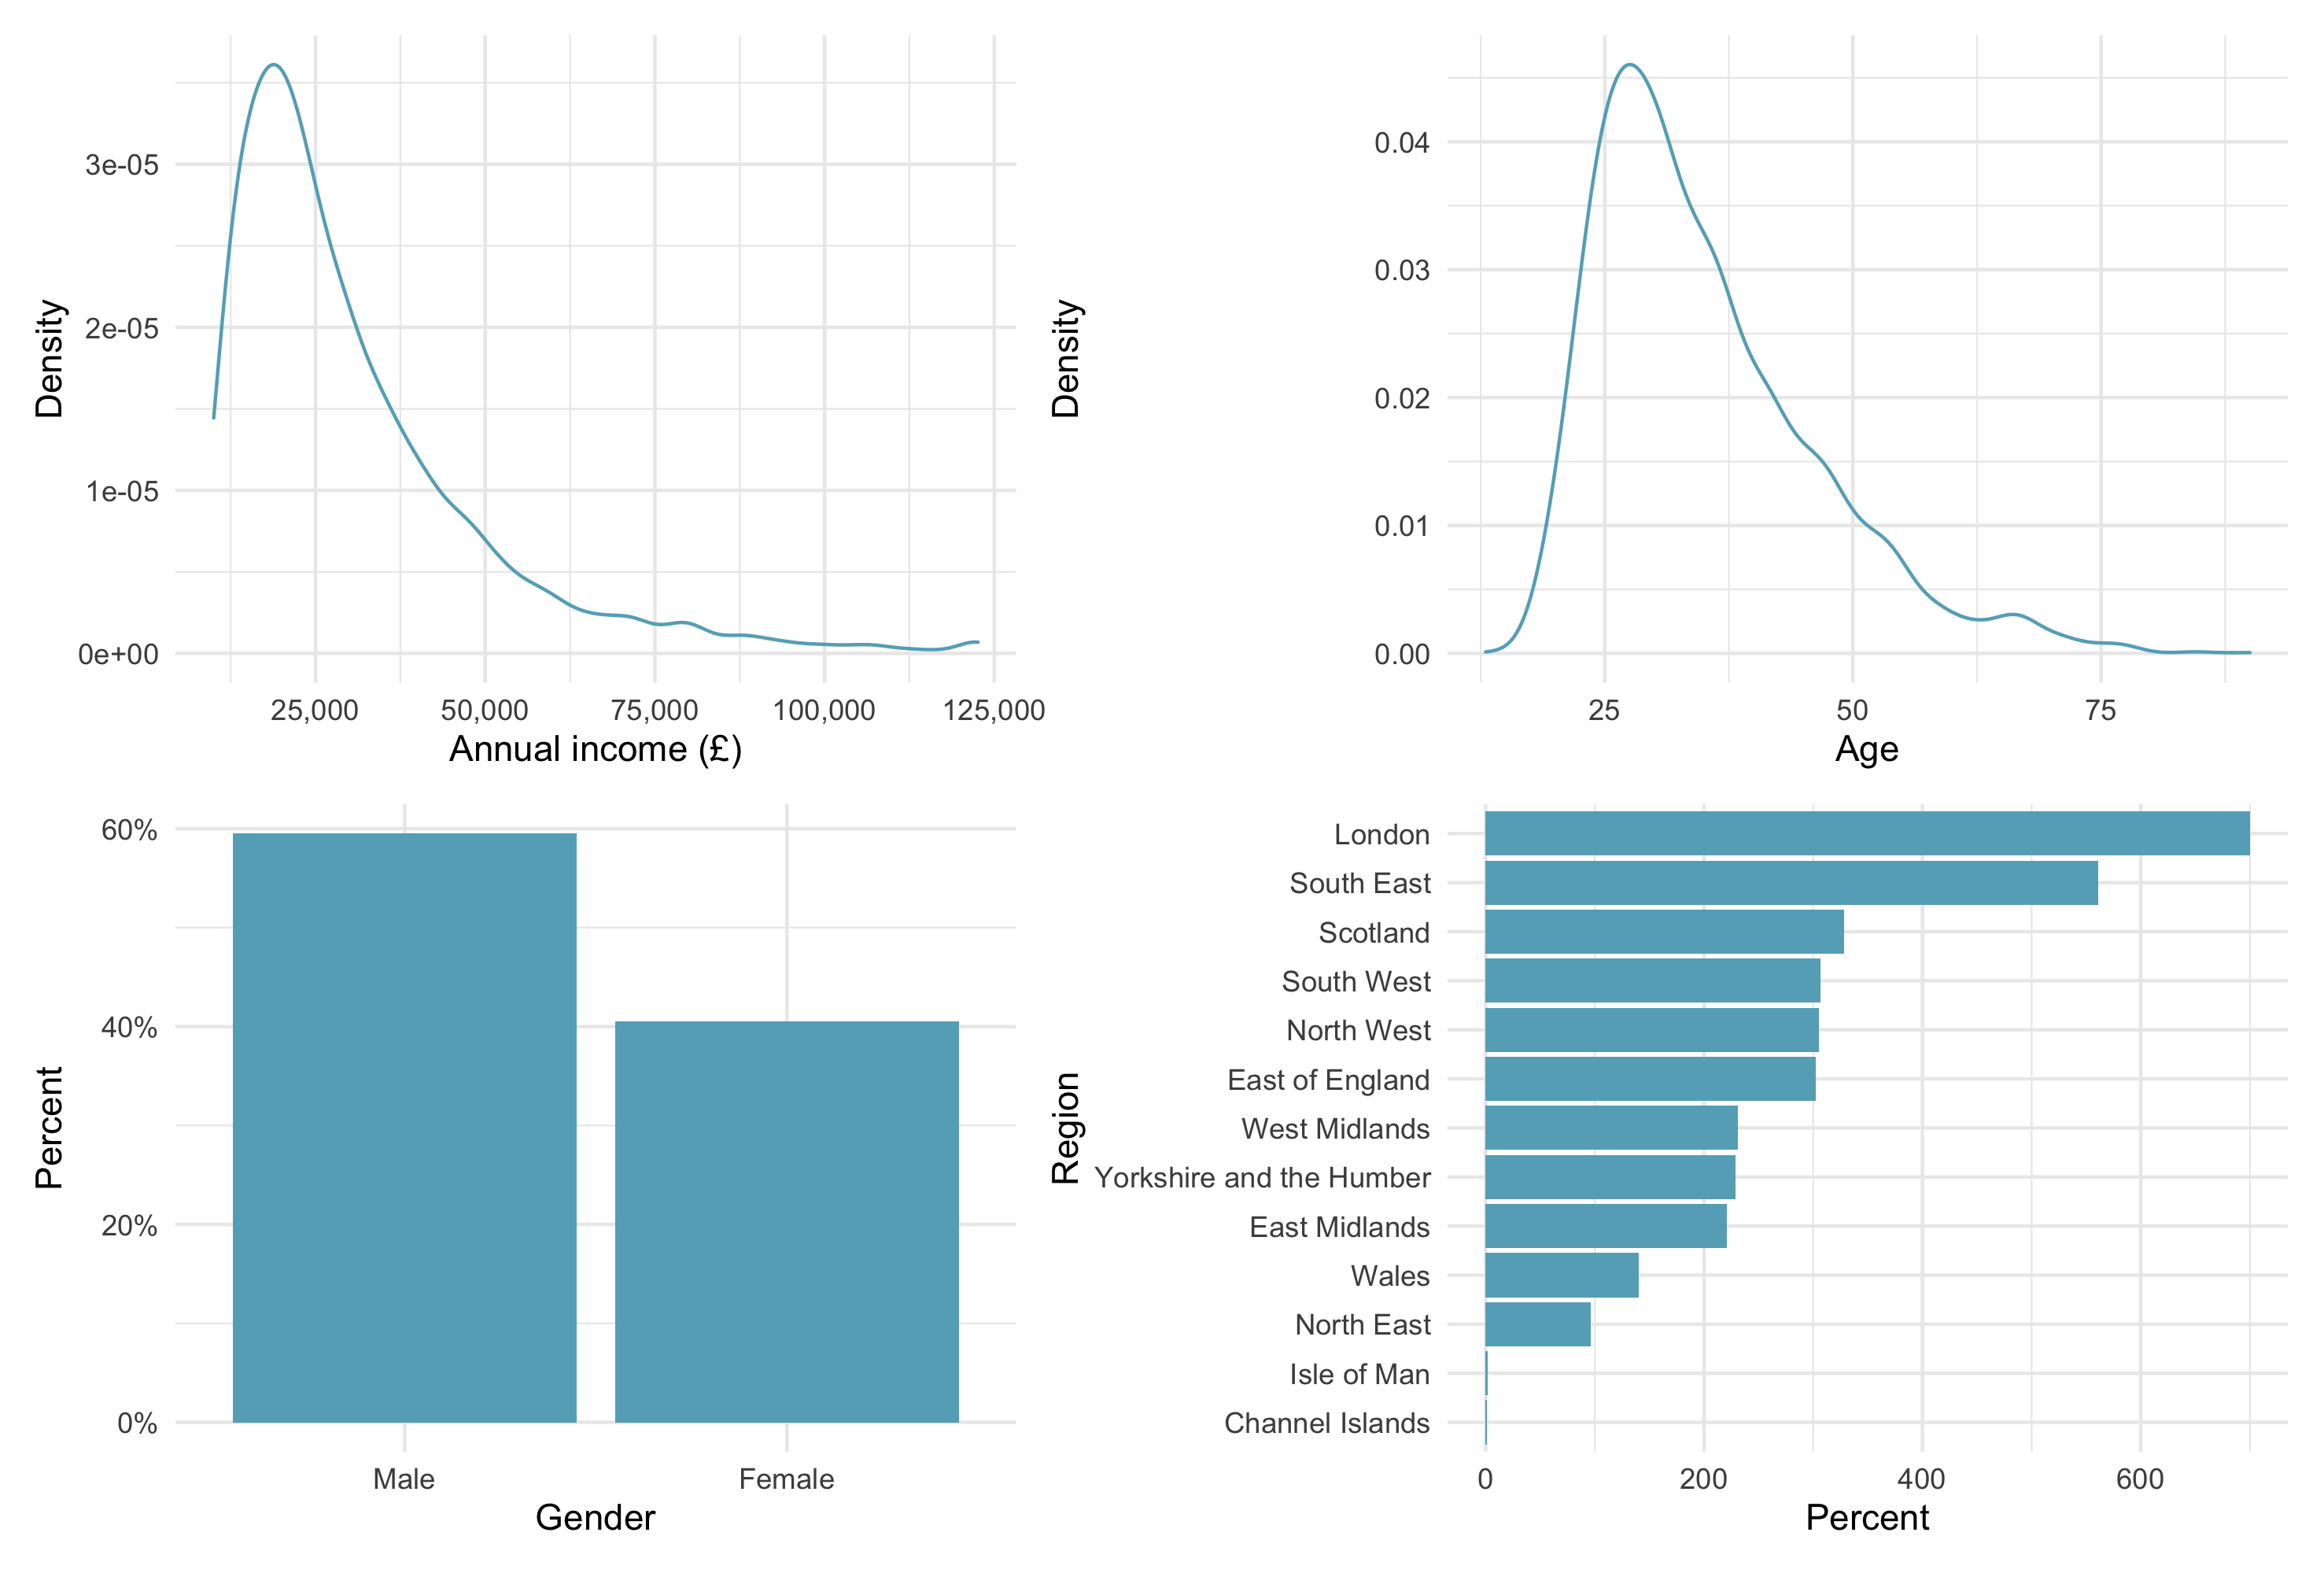
\includegraphics[width=.9\textwidth]{\figdir/sample_desc.png}
    \end{center}
\end{figure}

Figure~\ref{fig:entropy_kdes}
\begin{figure}[H]
    \center \newcommand\width{\textwidth} \caption{Entropy distributions}
    \label{fig:entropy_kdes}
    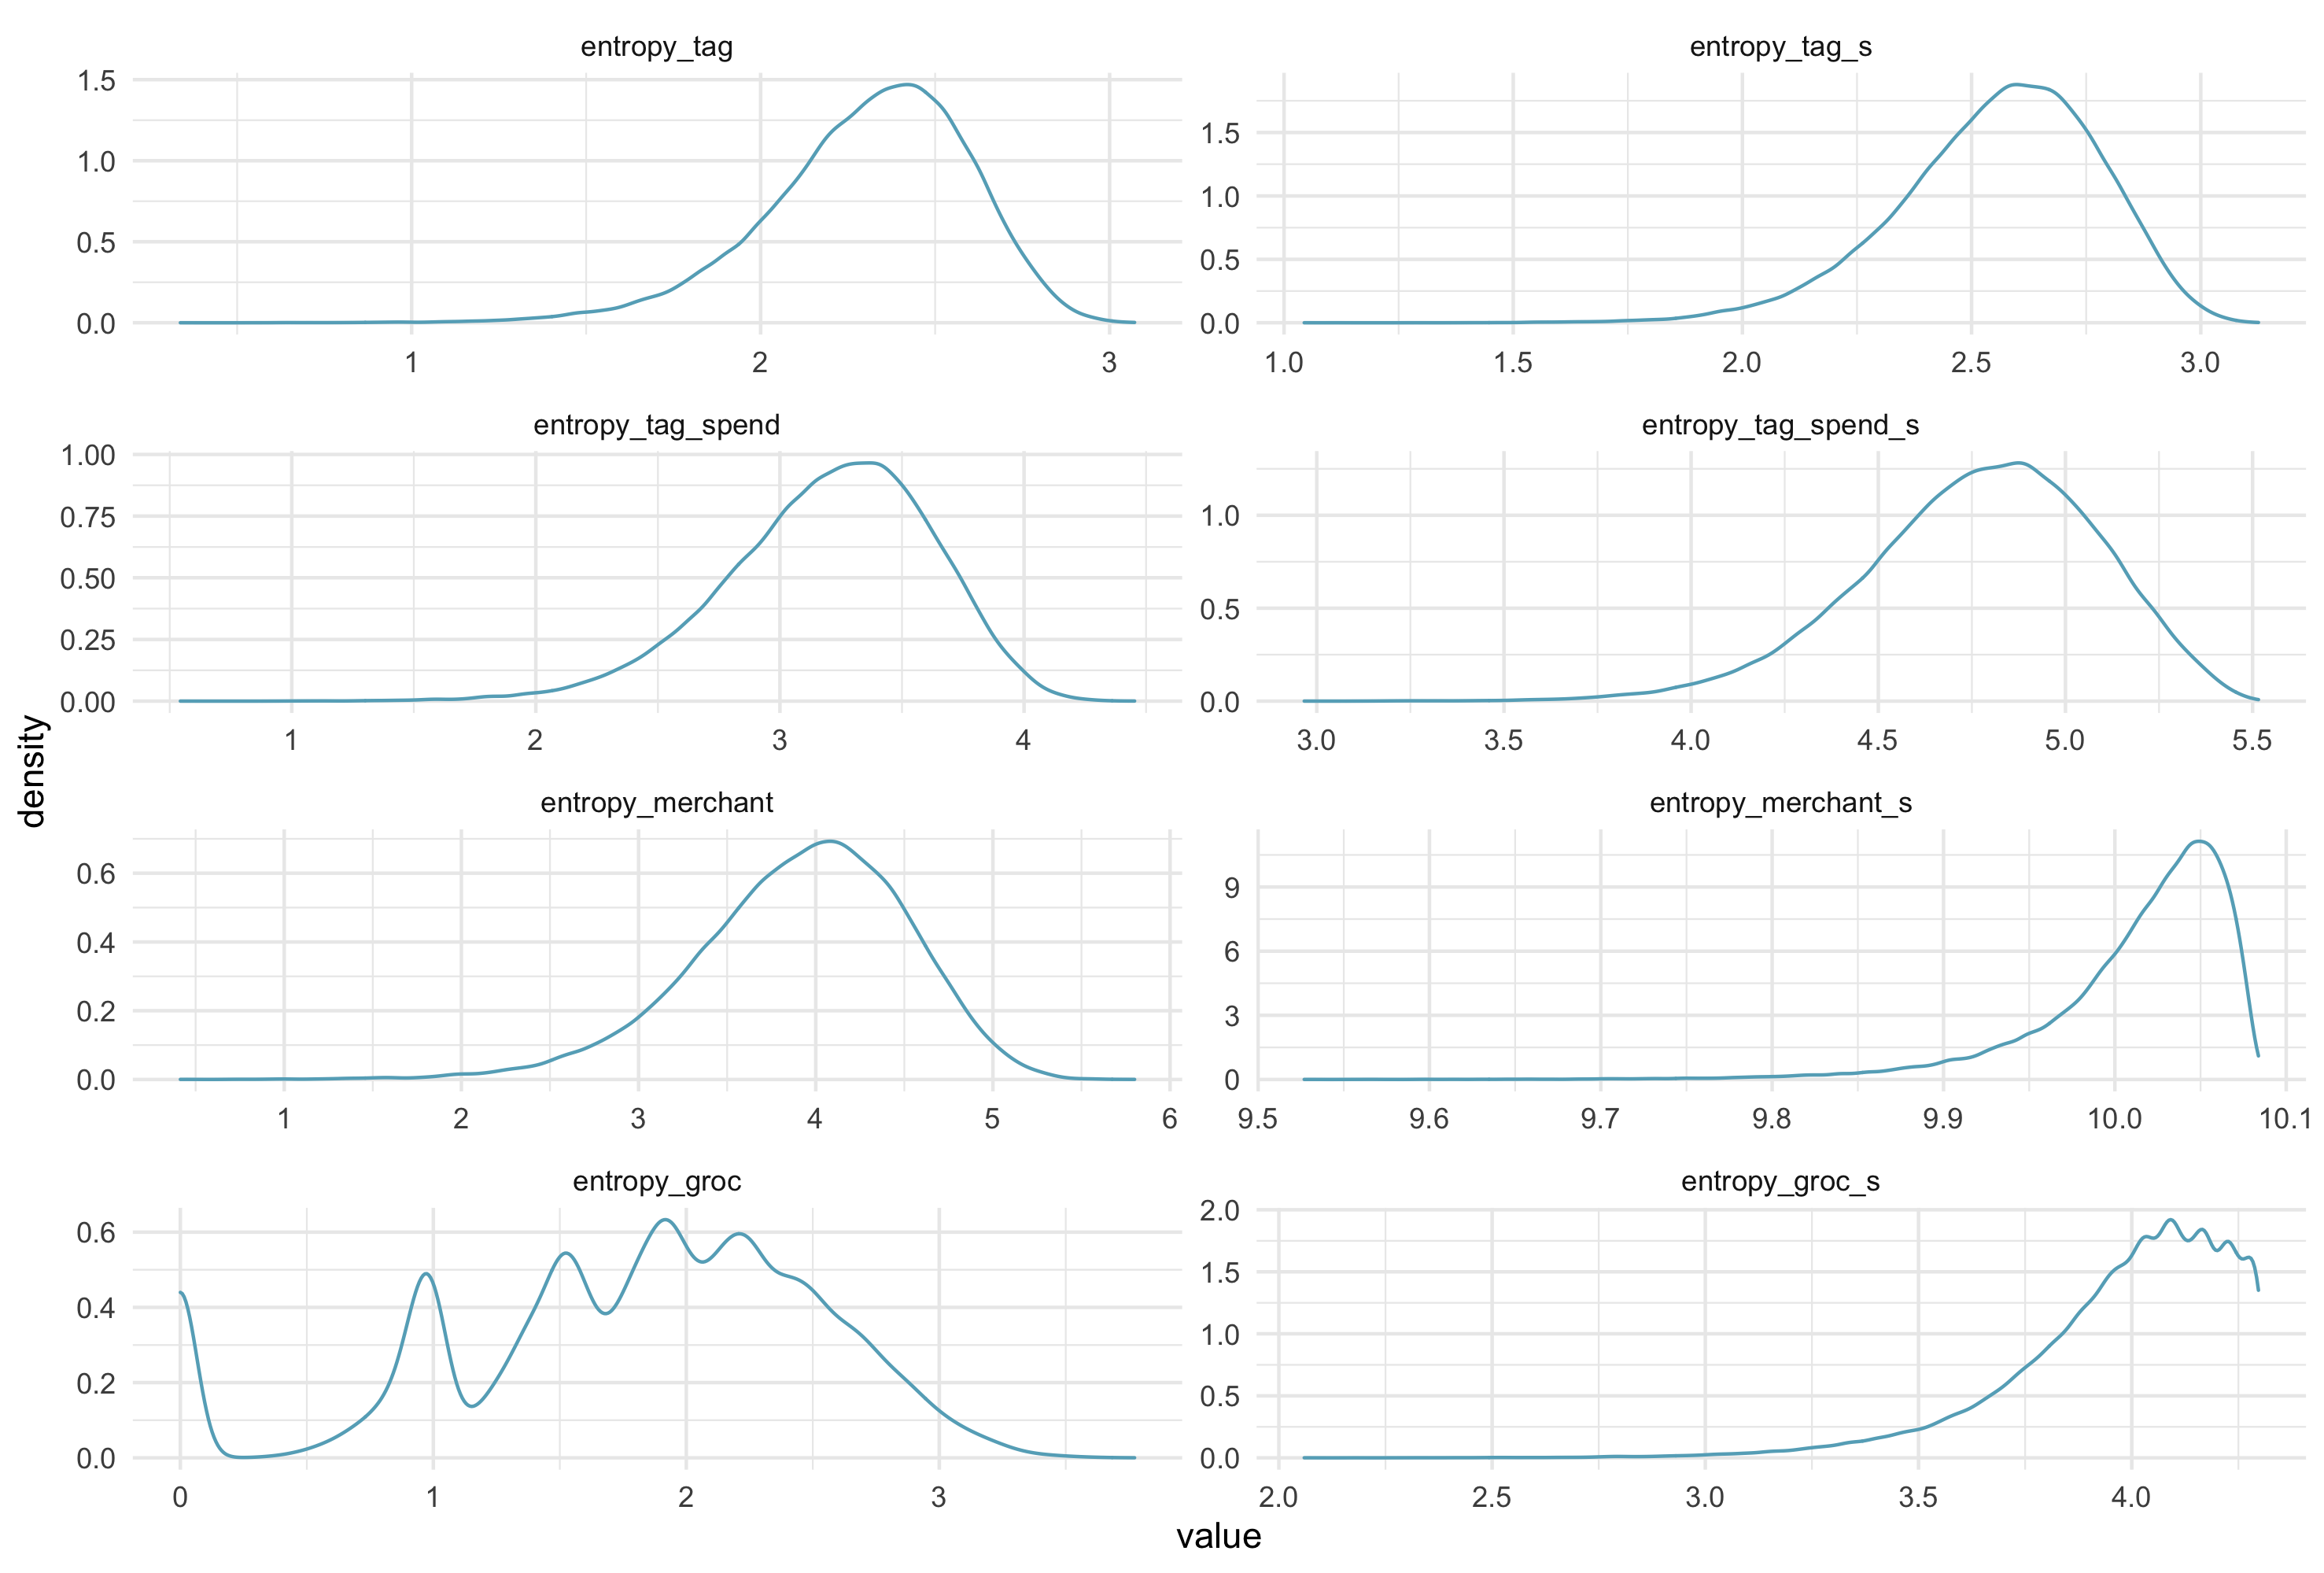
\includegraphics[width=\width]{\figdir/entropy_kdes.png}
    \fignote{\width}{}
\end{figure}


\subsection{Estimation}%
\label{sub:estimation}

We estimate models of the form: 

\begin{equation}
    y_{i,t} = \alpha_i + \lambda_t + \beta H_{i,t} + x^\prime_{i,t} \delta +
    \epsilon_{i,t},
\end{equation}

\noindent where $y_{i,t}$ is an indicator variable equal to one if individual $i$ made
one or more transfers to any of their savings account in year-month period $t$ and zero
otherwise, $H_{it}$ is $i$'s spending entropy in year-month period $t$, $x_{i,t}$ a vector
of control variables, $\alpha_i$ an individual fixed effect, $\lambda_t$ a
year-month fixed effect, and $\epsilon_{i, t}$ the error term.

The vector of controls includes month spend, month income, an indicator for
whether a user had positive income in a given month, and income
variability, calculated as the standard deviation of month income over the
previous 12 months.

Note that while we might in principle be worried about reverse causality, since
making payments into savings accounts might lead to a non-zero count in an
additional spend category and thus change entropy, this is not a concern here.
As discussed in Section~\ref{sub:dependent_variables} and
Section~\ref{sub:spending_profiles}, we define savings as inflows into savings
accounts and define entropy based on the classification of spend transactions
on current accounts. If a user pays money from their current into one of their
savings account, such a transaction will usually be labelled in their current
account as a transfer rather than a spending transaction, and thus not enter
the calculation of their entropy score. In Appendix~\ref{sub:endogeneity}, we
provide robustness checks using lagged entropy scores, which produces very
similar results.

